\documentclass{report}
\usepackage{fullpage}
\usepackage{graphicx}
\usepackage{float}
\renewcommand{\baselinestretch}{2}
\setlength{\parindent}{4em}
\setlength{\parskip}{1em}
\setcounter{secnumdepth}{0} % sections are level 1
\author{Nathan Morgenstern, Seo Bo Shim}
\title{Artificial Intelligence: Local Search}
\begin{document}
\maketitle
\tableofcontents


\newpage
\section{Introduction to the Graphical User Interface(GUI)}
When the Graphical User Interface starts up the user is able to select the type of puzzle evaluation through a drop down menu. The given options include: Basic Puzzle Evaluation, User Generated Puzzle Evaluation, Basic Hill Climbing, Hill Climbing with Random Restarts, Hill Climbing with Random Walk, Simulated Annealing, and Population Based Approach. 


	\begin{figure}[H]
	\centering
	\includegraphics[scale=0.50]{/Users/nathanmorgenstern/Desktop/aiImages/GUI/guiMain.png}
	\caption{Main Menu of GUI}
	\label{fig: Puzzle Evaluation Main Menu}
	\end{figure}


Each of the options then have their own corresponding window which is comprised of four main tabs: Puzzle Initialization, Puzzle, Puzzle Moves, and Data. The Puzzle Initialization tab is slightly different for each option in regards to the type of input received. The tabs Puzzle and Puzzle moves provide the user with a graphical representation of the generated puzzle as well as a graphical representation of the number of moves that it takes to get to each cell respectively.


\subsection{Basic Puzzle Evaluation}

	\begin{figure}[H]
	\centering
	\includegraphics[scale=0.41]{/Users/nathanmorgenstern/Desktop/aiImages/GUI/basiclnitialization.png}
	\caption{Puzzle Initialization of Basic Evaluation}
	\label{fig: Puzzle Initialization Tab of Basic Evaluation}
	\end{figure}

	\begin{figure}[H]
	\centering
	\includegraphics[scale=0.41]{/Users/nathanmorgenstern/Desktop/aiImages/GUI/basicPuzzle.png}
	\caption{Puzzle Tab of Basic Evaluation}
	\label{fig: Puzzle Tab of Basic Evaluation}
	\end{figure}

	\begin{figure}[H]
	\centering
	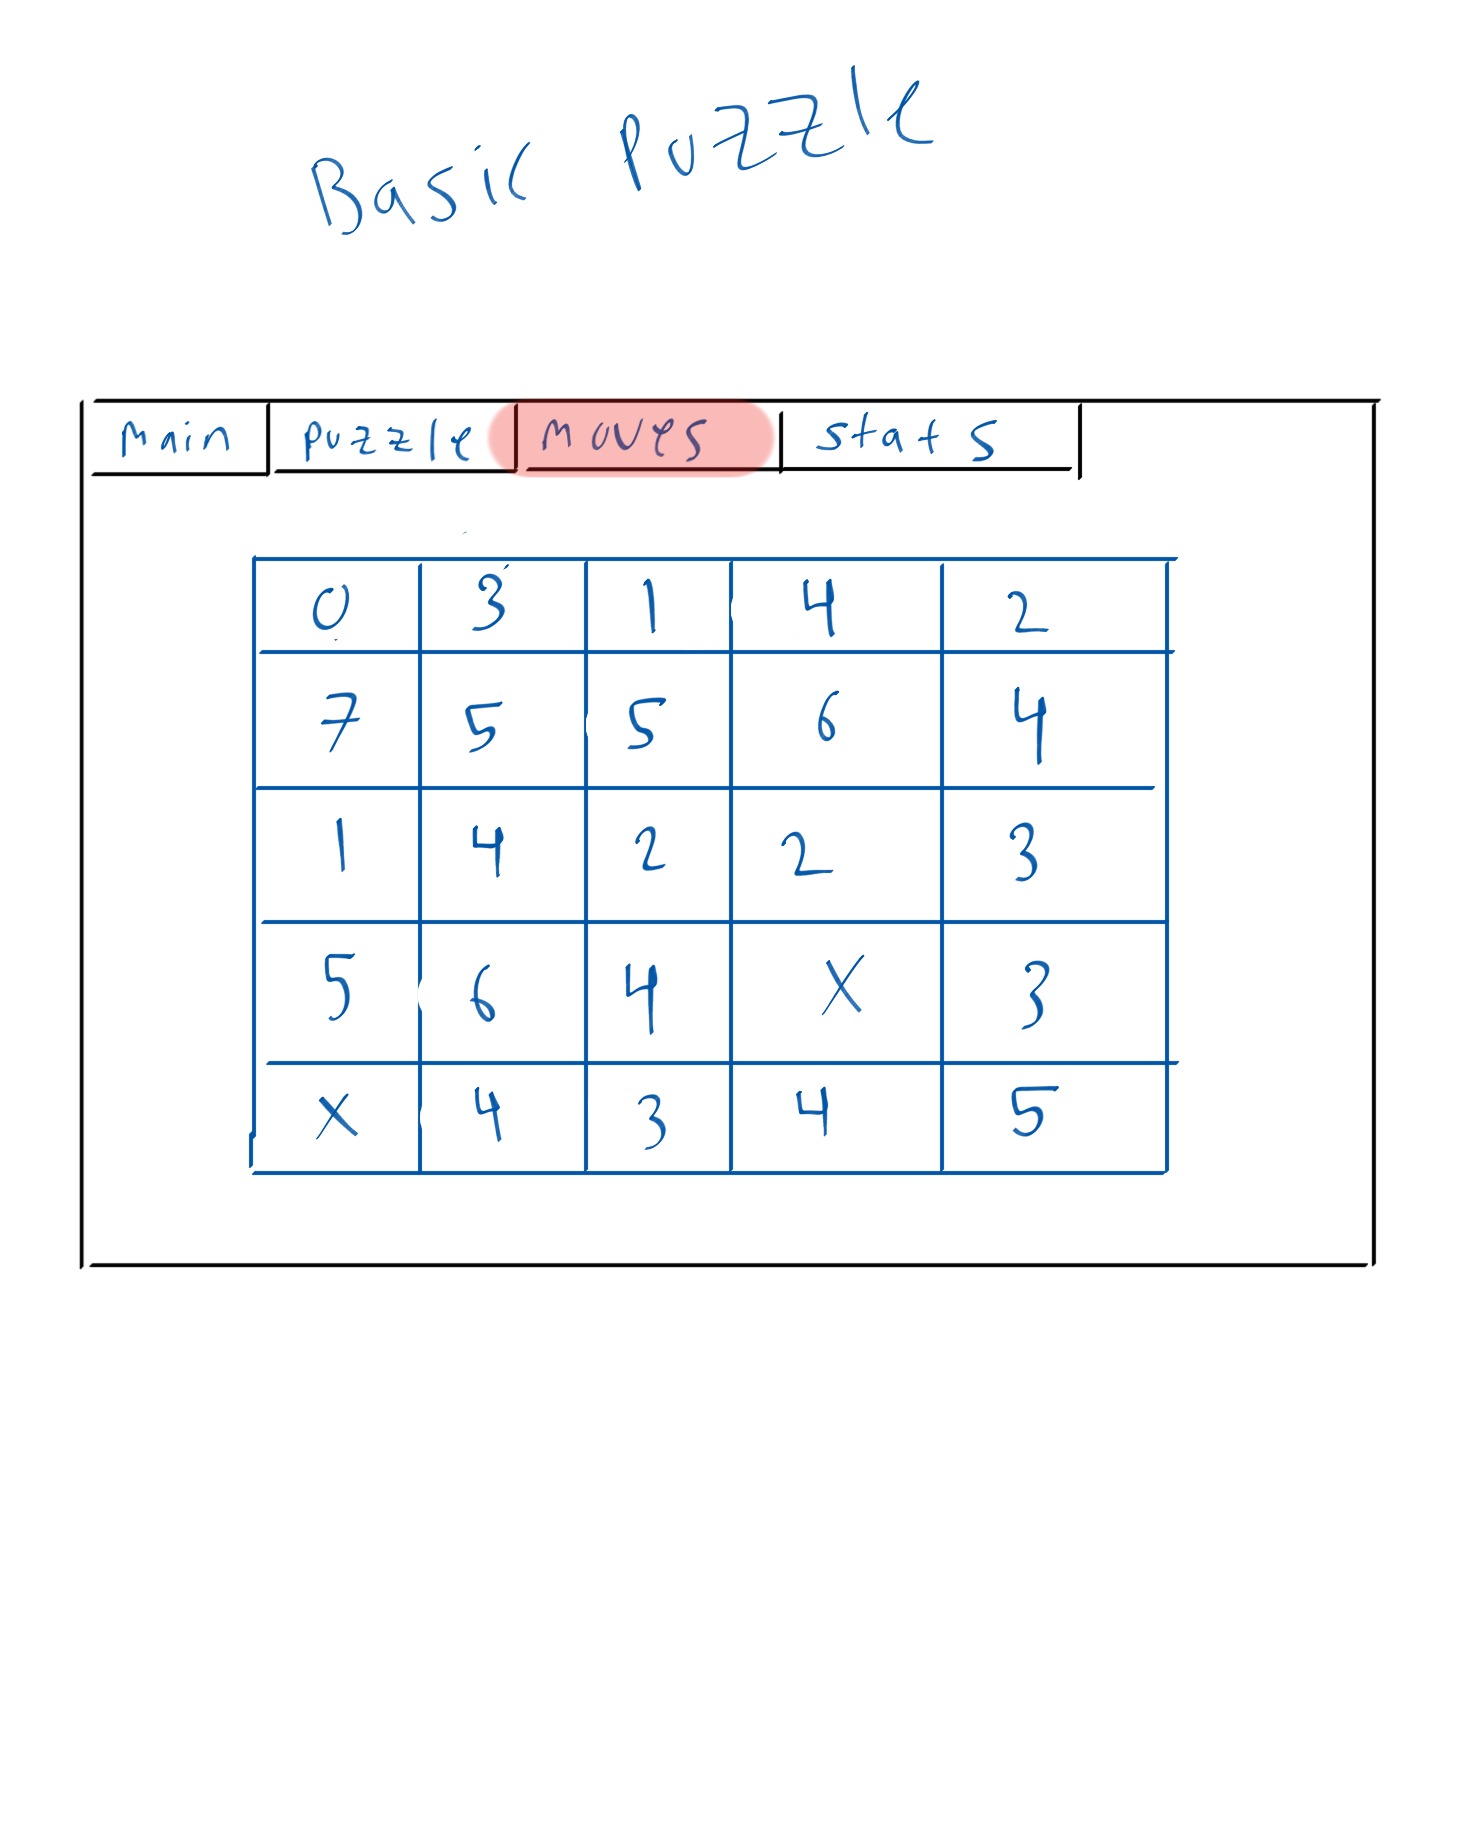
\includegraphics[scale=0.43]{/Users/nathanmorgenstern/Desktop/aiImages/GUI/basicPuzzleMoves.png}
	\caption{Puzzle Moves Tab of Basic Evaluation}
	\label{fig: Puzzle Moves Tab of Basic Evaluation}
	\end{figure}

	\begin{figure}[H]
	\centering
	\includegraphics[scale=0.43]{/Users/nathanmorgenstern/Desktop/aiImages/GUI/basicPuzzleEvaluation.png}
	\caption{Puzzle Data Tab of Basic Evaluation}
	\label{fig: Puzzle Data Tab of Basic Evaluation}
	\end{figure}

\subsection{User Generated Puzzle Evaluation}
The User Generated Puzzle Menu starts up with the default file of ./userPuzzles/assignment.txt, the user is able to change the file name to any location that they wish. The tabs Puzzle, Puzzle Moves, and Puzzle Evaluation are the same as the above examples for the Basic Puzzle Menu.

	\begin{figure}[H]
	\centering
	\includegraphics[scale=0.50]{/Users/nathanmorgenstern/Desktop/aiImages/GUI/userGeneratedInput.png}
	\caption{Puzzle Initialization Menu for User Generated Puzzle}
	\label{fig: Puzzle Initialization Menu for User Generated Puzzle}
	\end{figure}


\subsection{Basic Hill Climbing}
The Basic Hill Climbing Menu allows input for the size of the puzzle as well as a number of total iterations to perform the hill climbing algorithm. The data menu differs from the first two options in that it now shows a total evaluation time in addition to the evaluation function output.

	\begin{figure}[H]
	\centering
	\includegraphics[scale=0.50]{/Users/nathanmorgenstern/Desktop/aiImages/GUI/basicHillClimbingInput.png}
	\caption{Puzzle Initialization Menu for Basic Hill Climbing}
	\label{fig: Puzzle Initialization Menu for Basic Hill Climbing}
	\end{figure}
	
	\begin{figure}[H]
	\centering
	\includegraphics[scale=0.37]{/Users/nathanmorgenstern/Desktop/aiImages/GUI/basicHillClimbingEvaluation.png}
	\caption{Puzzle Evaluation Tab for Basic Hill Climbing}
	\label{fig: Puzzle Evaluation Tab for Basic Hill Climbing}
	\end{figure}

\subsection{Hill Climbing with Random Restarts}
The Hill Climbing with Random Restarts Menu is similiar to the Basic Hill Climbing menu, with the addition of an input option for the number of random restarts that should be performed. The Puzzle, Puzzle Moves, and Evaluation tabs remain unchanged from the previous example.

	\begin{figure}[H]
	\centering
	\includegraphics[scale=0.50]{/Users/nathanmorgenstern/Desktop/aiImages/GUI/hillClimbingRandomRestarts.png}
	\caption{Puzzle Initialization Menu for Hill Climbing with Random Restarts}
	\label{fig: Puzzle Initialization Menu for Hill Climbing with Random Restarts}
	\end{figure}
	
\newpage	
\subsection{Hill Climbing with Random Walk}
Hill Climbing with Random Walks Menu is the same as Hill Climbing with Random Restarts, but replaces the bottom input option of number of restarts, with the probability of down hill acceptance.

	\begin{figure}[H]
	\centering
	\includegraphics[scale=0.50]{/Users/nathanmorgenstern/Desktop/aiImages/GUI/hillClimbingRandomWalk.png}
	\caption{Puzzle Initialization Menu for Hill Climbing with Random Walk}
	\label{fig: Puzzle Initialization Menu for Hill Climbing with Random Walk}
	\end{figure}
	
\newpage	
\subsection{Simulated Annealing}
The initialization menu for Simulated Annealing includes 4 input options: the size n of the puzzle of the puzzle, the initial temperature T, the total number of iterations, and the decay rate.
 
	\begin{figure}[H]
	\centering
	\includegraphics[scale=0.50]{/Users/nathanmorgenstern/Desktop/aiImages/GUI/SA_menu.png}
	\caption{Puzzle Initialization Menu for Simulated Annealing}
	\label{fig: Puzzle Initialization Menu for Simulated Annealing}
	\end{figure}
	
\newpage	
\subsection{Population Based Approach}
The initialization menu for Populated Based Approach includes 4 input options: the size n of the puzzle of the puzzle, the computation time limit, the initial population size, and the probability for mutation.

	\begin{figure}[H]
	\centering
	\includegraphics[scale=0.50]{/Users/nathanmorgenstern/Desktop/aiImages/GUI/PA_menu.png}
	\caption{Puzzle Initialization Menu for Population Based Approach}
	\label{fig: Puzzle Initialization Menu for Population Based Approach}
	\end{figure}

\newpage
\section{Puzzle Evaluation}

In your report please include an example of 2 example puzzles for each size of n, where
one of the puzzles is solvable and the other is not solvable.

You will be asked during the demo to execute the evaluation puzzle on example puzzles and present the 
corresponding visualization. INCLUDE OPTION FOR FILE SELECTION?


\subsection{Example Puzzle for n = 5}

	\begin{figure}[H]
	\centering
	\includegraphics[scale=0.43]{/Users/nathanmorgenstern/Desktop/aiImages/basic/basic_size5_solvable_puzzlePane.png}
	\caption{Reachable Goal Puzzle size n = 5}
	\label{fig: Basic Evaluation n = 5 reachable goal puzzle }
	\end{figure}
	
	\begin{figure}[H]
	\centering
	\includegraphics[scale=0.43]{/Users/nathanmorgenstern/Desktop/aiImages/basic/basic_size5_solvable_puzzleMovesPane.png}
	\caption{Reachable Goal Puzzle Moves size n = 5}
	\label{fig: Basic Evaluation n = 5 reachable goal puzzle moves}
	\end{figure}
	
	\begin{figure}[H]
	\centering
	\includegraphics[scale=0.43]{/Users/nathanmorgenstern/Desktop/aiImages/basic/basic_size5_solvable_evalPane.png}
	\caption{Reachable Goal Puzzle Evaluation size n = 5}
	\label{fig: Basic Evaluation n = 5 reachable goal puzzle evaluation}
	\end{figure}
	
	\begin{figure}[H]
	\centering
	\includegraphics[scale=0.43]{/Users/nathanmorgenstern/Desktop/aiImages/basic/basic_size5_puzzlePane.png}
	\caption{Unreachable Goal Puzzle size n = 5}
	\label{fig: Basic Evaluation n = 5 unreachable goal puzzle }
	\end{figure}
	
	\begin{figure}[H]
	\centering
	\includegraphics[scale=0.43]{/Users/nathanmorgenstern/Desktop/aiImages/basic/basic_size5_puzzleMoves.png}
	\caption{Unreachable Goal Puzzle Moves size n = 5}
	\label{fig: Basic Evaluation n = 5 unreachable goal puzzle moves}
	\end{figure}
	
	\begin{figure}[H]
	\centering
	\includegraphics[scale=0.33]{/Users/nathanmorgenstern/Desktop/aiImages/basic/basic_size5_eval.png}
	\caption{Unreachable Goal Puzzle Evaluation size n = 5}
	\label{fig: Basic Evaluation n = 5 unreachable goal puzzle evaluation}
	\end{figure}
	
	
\subsection{Example Puzzle for n = 7}

	\begin{figure}[H]
	\centering
	\includegraphics[scale=0.40]{/Users/nathanmorgenstern/Desktop/aiImages/basic/basic_size7_solvable_puzzlePane.png}
	\caption{Reachable Goal Puzzle size n = 7}
	\label{fig: Basic Evaluation n = 7 reachable goal puzzle }
	\end{figure}
	
	\begin{figure}[H]
	\centering
	\includegraphics[scale=0.40]{/Users/nathanmorgenstern/Desktop/aiImages/basic/basic_size7_solvable_puzzleMovesPane.png}
	\caption{Reachable Goal Puzzle Moves size n = 7}
	\label{fig: Basic Evaluation n = 7 reachable goal puzzle moves}
	\end{figure}
	
	\begin{figure}[H]
	\centering
	\includegraphics[scale=0.40]{/Users/nathanmorgenstern/Desktop/aiImages/basic/basic_size7_solvable_evalPane.png}
	\caption{Reachable Goal Puzzle Evaluation size n = 7}
	\label{fig: Basic Evaluation n = 7 reachable goal puzzle evaluation}
	\end{figure}
	
	\begin{figure}[H]
	\centering
	\includegraphics[scale=0.43]{/Users/nathanmorgenstern/Desktop/aiImages/basic/basic_size7_puzzlePane.png}
	\caption{Unreachable Goal Puzzle size n = 7}
	\label{fig: Basic Evaluation n = 7 unreachable goal puzzle }
	\end{figure}
	
	\begin{figure}[H]
	\centering
	\includegraphics[scale=0.43]{/Users/nathanmorgenstern/Desktop/aiImages/basic/basic_size7_puzzleMoves.png}
	\caption{Unreachable Goal Puzzle Moves size n = 7}
	\label{fig: Basic Evaluation n = 7 unreachable goal puzzle moves}
	\end{figure}
	
	\begin{figure}[H]
	\centering
	\includegraphics[scale=0.33]{/Users/nathanmorgenstern/Desktop/aiImages/basic/basic_size7_eval.png}
	\caption{Unreachable Goal Puzzle Evaluation size n = 7}
	\label{fig: Basic Evaluation n = 7 unreachable goal puzzle evaluation}
	\end{figure}


\subsection{Example Puzzle for n = 9}

	\begin{figure}[H]
	\centering
	\includegraphics[scale=0.43]{/Users/nathanmorgenstern/Desktop/aiImages/basic/basic_size9_solvable_puzzlePane.png}
	\caption{Reachable Goal Puzzle size n = 9}
	\label{fig: Basic Evaluation n = 9 reachable goal puzzle }
	\end{figure}
	
	\begin{figure}[H]
	\centering
	\includegraphics[scale=0.43]{/Users/nathanmorgenstern/Desktop/aiImages/basic/basic_size9_solvable_puzzleMovesPane.png}
	\caption{Reachable Goal Puzzle Moves size n = 9}
	\label{fig: Basic Evaluation n = 9 reachable goal puzzle moves}
	\end{figure}
	
	\begin{figure}[H]
	\centering
	\includegraphics[scale=0.43]{/Users/nathanmorgenstern/Desktop/aiImages/basic/basic_size9_solvable_evalPane.png}
	\caption{Reachable Goal Puzzle Evaluation size n = 9}
	\label{fig: Basic Evaluation n = 9 reachable goal puzzle evaluation}
	\end{figure}
	
	\begin{figure}[H]
	\centering
	\includegraphics[scale=0.43]{/Users/nathanmorgenstern/Desktop/aiImages/basic/basic_size9_puzzlePane.png}
	\caption{Unreachable Goal Puzzle size n = 9}
	\label{fig: Basic Evaluation n = 9 unreachable goal puzzle }
	\end{figure}
	
	\begin{figure}[H]
	\centering
	\includegraphics[scale=0.43]{/Users/nathanmorgenstern/Desktop/aiImages/basic/basic_size9_puzzleMoves.png}
	\caption{Unreachable Goal Puzzle Moves size n = 9}
	\label{fig: Basic Evaluation n = 9 unreachable goal puzzle moves}
	\end{figure}
	
	\begin{figure}[H]
	\centering
	\includegraphics[scale=0.33]{/Users/nathanmorgenstern/Desktop/aiImages/basic/basic_size9_eval.png}
	\caption{Unreachable Goal Puzzle Evaluation size n = 9}
	\label{fig: Basic Evaluation n = 9 unreachable goal puzzle evaluation}
	\end{figure}


\subsection{Example Puzzle for n = 11}

	\begin{figure}[H]
	\centering
	\includegraphics[scale=0.43]{/Users/nathanmorgenstern/Desktop/aiImages/basic/basic_size11_solvable_puzzlePane.png}
	\caption{Reachable Goal Puzzle size n = 11}
	\label{fig: Basic Evaluation n = 11 reachable goal puzzle }
	\end{figure}
	
	\begin{figure}[H]
	\centering
	\includegraphics[scale=0.43]{/Users/nathanmorgenstern/Desktop/aiImages/basic/basic_size11_solvable_puzzleMovesPane.png}
	\caption{Reachable Goal Puzzle Moves size n = 11}
	\label{fig: Basic Evaluation n = 11 reachable goal puzzle moves}
	\end{figure}
	
	\begin{figure}[H]
	\centering
	\includegraphics[scale=0.43]{/Users/nathanmorgenstern/Desktop/aiImages/basic/basic_size11_solvable_evalPane.png}
	\caption{Reachable Goal Puzzle Evaluation size n = 11}
	\label{fig: Basic Evaluation n = 11 reachable goal puzzle evaluation}
	\end{figure}
	
	\begin{figure}[H]
	\centering
	\includegraphics[scale=0.43]{/Users/nathanmorgenstern/Desktop/aiImages/basic/basic_size11_puzzlePane.png}
	\caption{Unreachable Goal Puzzle size n = 11}
	\label{fig: Basic Evaluation n = 11 unreachable goal puzzle }
	\end{figure}
	
	\begin{figure}[H]
	\centering
	\includegraphics[scale=0.43]{/Users/nathanmorgenstern/Desktop/aiImages/basic/basic_size11_puzzleMoves.png}
	\caption{Unreachable Goal Puzzle Moves size n = 11}
	\label{fig: Basic Evaluation n = 11 unreachable goal puzzle moves}
	\end{figure}
	
	\begin{figure}[H]
	\centering
	\includegraphics[scale=0.43]{/Users/nathanmorgenstern/Desktop/aiImages/basic/basic_size11_eval.png}
	\caption{Unreachable Goal Puzzle Evaluation size n = 11}
	\label{fig: Basic Evaluation n = 11 unreachable goal puzzle evaluation}
	\end{figure}


\section{Basic Hill Climbing Approach}
Your software should receive the number of iterations for the hill climbing approach as input and visualize the final optimized puzzle configuration, its value and the time it took to compute it.

\subsection{Example Puzzle for n = 5}

	\begin{figure}[H]
	\centering
	\includegraphics[scale=0.40]{/Users/nathanmorgenstern/Desktop/aiImages/basicHillClimbing/basicHillClimbingPuzzle_size5.png}
	\caption{Basic Hill Climbing Best Puzzle after 100,000 iterations for n = 5} 
	\label{fig: Basic Hill Climbing Best Puzzle after 100,000 iterations for n = 5}
	\end{figure}
	
	\begin{figure}[H]
	\centering
	\includegraphics[scale=0.40]{/Users/nathanmorgenstern/Desktop/aiImages/basicHillClimbing/basicHillClimbingPuzzleMoves_size5.png}
	\caption{Basic Hill Climbing Puzzle Moves  after 100,000 iterations for n = 5} 
	\label{fig: Basic Hill Climbing Puzzle Moves after 100,000 iterations for n = 5}
	\end{figure}

	\begin{figure}[H]
	\centering
	\includegraphics[scale=0.31]{/Users/nathanmorgenstern/Desktop/aiImages/basicHillClimbing/basicHillClimbingEvaluation_size5.png}
	\caption{Basic Hill Climbing Puzzle Evaluation after 100,000 iterations for n = 5} 
	\label{fig: Basic Hill Climbing Puzzle Evaluation after 100,000 iterations for n = 5}
	\end{figure}
	
	\begin{figure}[H]
	\centering
	\includegraphics[scale=0.40]{/Users/nathanmorgenstern/Desktop/aiImages/basicHillClimbing/basicHillClimbingPlot_50trials_1000_iterations_size5}
	\caption{Plot of 100,000 iterations averaged over 50 runs for n = 5} 
	\label{fig: Plot of 100,000 iterations averaged over 50 runs for n = 5}
	\end{figure}

\subsection{Example Puzzle for n = 7}

	\begin{figure}[H]
	\centering
	\includegraphics[scale=0.40]{/Users/nathanmorgenstern/Desktop/aiImages/basicHillClimbing/basicHillClimbingPuzzle_size7.png}
	\caption{Basic Hill Climbing Best Puzzle after 100,000 iterations for n = 7} 
	\label{fig: Basic Hill Climbing Best Puzzle after 100,000 iterations for n = 7}
	\end{figure}
	
	\begin{figure}[H]
	\centering
	\includegraphics[scale=0.40]{/Users/nathanmorgenstern/Desktop/aiImages/basicHillClimbing/basicHillClimbingPuzzleMoves_size7.png}
	\caption{Basic Hill Climbing Puzzle Moves  after 100,000 iterations for n = 7} 
	\label{fig: Basic Hill Climbing Puzzle Moves after 100,000 iterations for n = 7}
	\end{figure}

	\begin{figure}[H]
	\centering
	\includegraphics[scale=0.31]{/Users/nathanmorgenstern/Desktop/aiImages/basicHillClimbing/basicHillClimbingEvaluation_size7.png}
	\caption{Basic Hill Climbing Puzzle Evaluation after 100,000 iterations for n = 7} 
	\label{fig: Basic Hill Climbing Puzzle Evaluation after 100,000 iterations for n = 7}
	\end{figure}
	
	\begin{figure}[H]
	\centering
	\includegraphics[scale=0.40]{/Users/nathanmorgenstern/Desktop/aiImages/basicHillClimbing/basicHillClimbingPlot_50trials_1000_iterations_size7}
	\caption{Plot of 100,000 iterations averaged over 50 runs for n = 7}
	\label{fig: Plot of 100,000 iterations averaged over 50 runs for n = 7}
	\end{figure}
	
\subsection{Example Puzzle for n = 9}
	
	\begin{figure}[H]
	\centering
	\includegraphics[scale=0.40]{/Users/nathanmorgenstern/Desktop/aiImages/basicHillClimbing/basicHillClimbingPuzzle_size9.png}
	\caption{Basic Hill Climbing Best Puzzle after 100,000 iterations for n = 9} 
	\label{fig: Basic Hill Climbing Best Puzzle after 100,000 iterations for n = 9}
	\end{figure}
	
	\begin{figure}[H]
	\centering
	\includegraphics[scale=0.40]{/Users/nathanmorgenstern/Desktop/aiImages/basicHillClimbing/basicHillClimbingPuzzleMoves_size9.png}
	\caption{Basic Hill Climbing Puzzle Moves  after 100,000 iterations for n = 9} 
	\label{fig: Basic Hill Climbing Puzzle Moves after 100,000 iterations for n = 9}
	\end{figure}

	\begin{figure}[H]
	\centering
	\includegraphics[scale=0.31]{/Users/nathanmorgenstern/Desktop/aiImages/basicHillClimbing/basicHillClimbingEvaluation_size9.png}
	\caption{Basic Hill Climbing Puzzle Evaluation after 100,000 iterations for n = 9} 
	\label{fig: Basic Hill Climbing Puzzle Evaluation after 100,000 iterations for n = 9}
	\end{figure}
	
	\begin{figure}[H]
	\centering
	\includegraphics[scale=0.40]{/Users/nathanmorgenstern/Desktop/aiImages/basicHillClimbing/basicHillClimbingPlot_50trials_1000_iterations_size9}
	\caption{Plot of 100,000 iterations averaged over 50 runs for n = 9}
	\label{fig: Plot of 100,000 iterations averaged over 50 runs for n = 9}
	\end{figure}
	
\subsection{Example Puzzle for n = 11}

	\begin{figure}[H]
	\centering
	\includegraphics[scale=0.40]{/Users/nathanmorgenstern/Desktop/aiImages/basicHillClimbing/basicHillClimbingPuzzle_size11.png}
	\caption{Basic Hill Climbing Best Puzzle after 100,000 iterations for n = 11} 
	\label{fig: Basic Hill Climbing Best Puzzle after 100,000 iterations for n = 11}
	\end{figure}
	
	\begin{figure}[H]
	\centering
	\includegraphics[scale=0.40]{/Users/nathanmorgenstern/Desktop/aiImages/basicHillClimbing/basicHillClimbingPuzzleMoves_size11.png}
	\caption{Basic Hill Climbing Puzzle Moves  after 100,000 iterations for n = 11} 
	\label{fig: Basic Hill Climbing Puzzle Moves after 100,000 iterations for n = 11}
	\end{figure}

	\begin{figure}[H]
	\centering
	\includegraphics[scale=0.31]{/Users/nathanmorgenstern/Desktop/aiImages/basicHillClimbing/basicHillClimbingEvaluation_size11.png}
	\caption{Basic Hill Climbing Puzzle Evaluation after 100,000 iterations for n = 11} 
	\label{fig: Basic Hill Climbing Puzzle Evaluation after 100,000 iterations for n = 11}
	\end{figure}

	\begin{figure}[H]
	\centering
	\includegraphics[scale=0.40]{/Users/nathanmorgenstern/Desktop/aiImages/basicHillClimbing/basicHillClimbingPlot_50trials_1000_iterations_size11}
	\caption{Plot of 100,000 iterations averaged over 50 runs for n = 11}
	\label{fig: Plot of 100,000 iterations averaged over 50 runs for n = 11}
	\end{figure}

\newpage
\section{Hill Climbing with Random Restarts}
The following puzzles were generated with 10,000 iterations and 10 restarts for a total of 100,000 iterations. The results are relatively similar to those of the standard 

\subsection{Example Puzzle for n = 5}

	\begin{figure}[H]
	\centering
	\includegraphics[scale=0.40]{/Users/nathanmorgenstern/Desktop/aiImages/hillClimbingRestarts/hillClimbingRestarts_size5.png}
	\caption{Hill Climbing with Random Restarts Best Puzzle after 100,000 iterations for n = 5} 
	\label{fig: Hill Climbing with Random Restarts Best Puzzle after 100,000 iterations for n = 5}
	\end{figure}
	
	\begin{figure}[H]
	\centering
	\includegraphics[scale=0.40]{/Users/nathanmorgenstern/Desktop/aiImages/hillClimbingRestarts/hillClimbingRestarts_move_size5.png}
	\caption{Hill Climbing with Random Restarts Best Puzzle after 100,000 iterations for n = 5} 
	\label{fig: Hill Climbing with Random Restarts Best Puzzle after 100,000 iterations for n = 5}
	\end{figure}

	\begin{figure}[H]
	\centering
	\includegraphics[scale=0.31]{/Users/nathanmorgenstern/Desktop/aiImages/hillClimbingRestarts/hillClimbingRestarts_eval_size5.png}
	\caption{Hill Climbing with Random Restarts Best Puzzle after 100,000 iterations for n = 5} 
	\label{fig: Hill Climbing with Random Restarts Best Puzzle after 100,000 iterations for n = 5}
	\end{figure}

	\begin{figure}[H]
	\centering
	\includegraphics[scale=0.40]{/Users/nathanmorgenstern/Desktop/aiImages/hillClimbingRestarts/hillClimbingRestartsPlot_50trials_size5.png}
	\caption{Plot of 100,000 iterations averaged over 50 runs for n = 5}
	\label{fig: Plot of 100,000 iterations averaged over 50 runs for n = 5}
	\end{figure}

\subsection{Example Puzzle for n = 7}

	\begin{figure}[H]
	\centering
	\includegraphics[scale=0.40]{/Users/nathanmorgenstern/Desktop/aiImages/hillClimbingRestarts/hillClimbingRestarts_size7.png}
	\caption{Hill Climbing with Random Restarts Best Puzzle after 100,000 iterations for n = 7} 
	\label{fig: Hill Climbing with Random Restarts Best Puzzle after 100,000 iterations for n = 7}
	\end{figure}
	
	\begin{figure}[H]
	\centering
	\includegraphics[scale=0.40]{/Users/nathanmorgenstern/Desktop/aiImages/hillClimbingRestarts/hillClimbingRestarts_moves_size7.png}
	\caption{Hill Climbing with Random Restarts Best Puzzle after 100,000 iterations for n = 7} 
	\label{fig: Hill Climbing with Random Restarts Best Puzzle after 100,000 iterations for n = 7}
	\end{figure}

	\begin{figure}[H]
	\centering
	\includegraphics[scale=0.31]{/Users/nathanmorgenstern/Desktop/aiImages/hillClimbingRestarts/hillClimbingRestarts_eval_size7.png}
	\caption{Hill Climbing with Random Restarts Best Puzzle after 100,000 iterations for n = 7} 
	\label{fig: Hill Climbing with Random Restarts Best Puzzle after 100,000 iterations for n = 7}
	\end{figure}

	\begin{figure}[H]
	\centering
	\includegraphics[scale=0.40]{/Users/nathanmorgenstern/Desktop/aiImages/hillClimbingRestarts/hillClimbingRestartsPlot_50trials_size7.png}
	\caption{Plot of 100,000 iterations averaged over 50 runs for n = 7}
	\label{fig: Plot of 100,000 iterations averaged over 50 runs for n = 7}
	\end{figure}
	
\subsection{Example Puzzle for n = 9}
\begin{figure}[H]
	\centering
	\includegraphics[scale=0.40]{/Users/nathanmorgenstern/Desktop/aiImages/hillClimbingRestarts/hillClimbingRestarts_size9.png}
	\caption{Hill Climbing with Random Restarts Best Puzzle after 100,000 iterations for n = 9} 
	\label{fig: Hill Climbing with Random Restarts Best Puzzle after 100,000 iterations for n = 9}
	\end{figure}
	
	\begin{figure}[H]
	\centering
	\includegraphics[scale=0.40]{/Users/nathanmorgenstern/Desktop/aiImages/hillClimbingRestarts/hillClimbingRestarts_moves_size9.png}
	\caption{Hill Climbing with Random Restarts Best Puzzle after 100,000 iterations for n = 9} 
	\label{fig: Hill Climbing with Random Restarts Best Puzzle after 100,000 iterations for n = 9}
	\end{figure}

	\begin{figure}[H]
	\centering
	\includegraphics[scale=0.31]{/Users/nathanmorgenstern/Desktop/aiImages/hillClimbingRestarts/hillClimbingRestarts_eval_size9.png}
	\caption{Hill Climbing with Random Restarts Best Puzzle after 100,000 iterations for n = 9} 
	\label{fig: Hill Climbing with Random Restarts Best Puzzle after 100,000 iterations for n = 9}
	\end{figure}

	\begin{figure}[H]
	\centering
	\includegraphics[scale=0.40]{/Users/nathanmorgenstern/Desktop/aiImages/hillClimbingRestarts/hillClimbingRestartsPlot_50trials_size9.png}
	\caption{Plot of 100,000 iterations averaged over 50 runs for n = 9}
	\label{fig: Plot of 100,000 iterations averaged over 50 runs for n = 9}
	\end{figure}
\subsection{Example Puzzle for n = 11}

	\begin{figure}[H]
	\centering
	\includegraphics[scale=0.40]{/Users/nathanmorgenstern/Desktop/aiImages/hillClimbingRestarts/hillClimbingRestarts_size11.png}
	\caption{Hill Climbing with Random Restarts Best Puzzle after 100,000 iterations for n = 11} 
	\label{fig: Hill Climbing with Random Restarts Best Puzzle after 100,000 iterations for n = 11}
	\end{figure}
	
	\begin{figure}[H]
	\centering
	\includegraphics[scale=0.40]{/Users/nathanmorgenstern/Desktop/aiImages/hillClimbingRestarts/hillClimbingRestarts_moves_size11.png}
	\caption{Hill Climbing with Random Restarts Best Puzzle after 100,000 iterations for n = 11} 
	\label{fig: Hill Climbing with Random Restarts Best Puzzle after 100,000 iterations for n = 11}
	\end{figure}

	\begin{figure}[H]
	\centering
	\includegraphics[scale=0.31]{/Users/nathanmorgenstern/Desktop/aiImages/hillClimbingRestarts/hillClimbingRestarts_eval_size11.png}
	\caption{Hill Climbing with Random Restarts Best Puzzle after 100,000 iterations for n = 11} 
	\label{fig: Hill Climbing with Random Restarts Best Puzzle after 100,000 iterations for n = 11}
	\end{figure}

	\begin{figure}[H]
	\centering
	\includegraphics[scale=0.40]{/Users/nathanmorgenstern/Desktop/aiImages/hillClimbingRestarts/hillClimbingRestartsPlot_50trials_size11.png}
	\caption{Plot of 100,000 iterations averaged over 50 runs for n = 11}
	\label{fig: Plot of 100,000 iterations averaged over 50 runs for n = 11}
	\end{figure}

\newpage
\section{Hill Climbing with Random Walks}
There were a total of 100,000 iterations run for each of the puzzle sizes with a probability of lower acceptance set at 0.03. The higher the probability of lower acceptance the worse the results tended to be.

\subsection{Example Puzzle for n = 5}


\subsection{Example Puzzle for n = 7}
IMAGES
\subsection{Example Puzzle for n = 9}
IMAGES
\subsection{Example Puzzle for n = 11}
IIMAGES

\newpage
\section{Simulated Annealing}

\subsection{Example Puzzle for n = 5}

	\begin{figure}[H]
	\centering
	\includegraphics[scale=0.40]{/Users/nathanmorgenstern/Desktop/aiImages/SimulatedAnnealing/SimulatedAnnealing_size5.png}
	\caption{Simulated Annealing Best Puzzle after 100,000 iterations for n = 5} 
	\label{fig: Simulated Annealing Best Puzzle after 100,000 iterations for n = 5}
	\end{figure}
	
	\begin{figure}[H]
	\centering
	\includegraphics[scale=0.40]{/Users/nathanmorgenstern/Desktop/aiImages/SimulatedAnnealing/SimulatedAnnealing_moves_size5.png}
	\caption{Simulated Annealing Best Puzzle Moves after 100,000 iterations for n = 5} 
	\label{fig: Simulated Annealing Best Puzzle Moves after 100,000 iterations for n = 5}
	\end{figure}

	\begin{figure}[H]
	\centering
	\includegraphics[scale=0.31]{/Users/nathanmorgenstern/Desktop/aiImages/SimulatedAnnealing/SimulatedAnnealing_eval_size5.png}
	\caption{Simulated Annealing Best Puzzle Evaluation after 100,000 iterations for n = 5} 
	\label{fig: Simulated Annealing Best Puzzle Evaluation after 100,000 iterations for n = 5} 
	\end{figure}

	\begin{figure}[H]
	\centering
	\includegraphics[scale=0.40]{/Users/nathanmorgenstern/Desktop/aiImages/SimulatedAnnealing/SimulatedAnnealingPlot_50trials_size5.png}
	\caption{Plot of 100,000 iterations averaged over 50 runs for n = 5}
	\label{fig: Plot of 100,000 iterations averaged over 50 runs for n = 5}
	\end{figure}

\subsection{Example Puzzle for n = 7}

	\begin{figure}[H]
	\centering
	\includegraphics[scale=0.40]{/Users/nathanmorgenstern/Desktop/aiImages/SimulatedAnnealing/SimulatedAnnealing_size7.png}
	\caption{Simulated Annealing Best Puzzle after 100,000 iterations for n = 7} 
	\label{fig: Simulated Annealing Best Puzzle after 100,000 iterations for n = 7}
	\end{figure}
	
	\begin{figure}[H]
	\centering
	\includegraphics[scale=0.40]{/Users/nathanmorgenstern/Desktop/aiImages/SimulatedAnnealing/SimulatedAnnealing_moves_size7.png}
	\caption{Simulated Annealing Best Puzzle Moves after 100,000 iterations for n = 7} 
	\label{fig: Simulated Annealing Best Puzzle Moves after 100,000 iterations for n = 7}
	\end{figure}

	\begin{figure}[H]
	\centering
	\includegraphics[scale=0.31]{/Users/nathanmorgenstern/Desktop/aiImages/SimulatedAnnealing/SimulatedAnnealing_eval_size7.png}
	\caption{Simulated Annealing Best Puzzle Evaluation after 100,000 iterations for n = 7} 
	\label{fig: Simulated Annealing Best Puzzle Evaluation after 100,000 iterations for n = 7} 
	\end{figure}

	\begin{figure}[H]
	\centering
	\includegraphics[scale=0.40]{/Users/nathanmorgenstern/Desktop/aiImages/SimulatedAnnealing/SimulatedAnnealingPlot_50trials_size7.png}
	\caption{Plot of 100,000 iterations averaged over 50 runs for n = 7}
	\label{fig: Plot of 100,000 iterations averaged over 50 runs for n = 7}
	\end{figure}


\subsection{Example Puzzle for n = 9}
	
	\begin{figure}[H]
	\centering
	\includegraphics[scale=0.40]{/Users/nathanmorgenstern/Desktop/aiImages/SimulatedAnnealing/SimulatedAnnealing_size9.png}
	\caption{Simulated Annealing Best Puzzle after 100,000 iterations for n = 9} 
	\label{fig: Simulated Annealing Best Puzzle after 100,000 iterations for n = 9}
	\end{figure}
	
	\begin{figure}[H]
	\centering
	\includegraphics[scale=0.40]{/Users/nathanmorgenstern/Desktop/aiImages/SimulatedAnnealing/SimulatedAnnealing_moves_size9.png}
	\caption{Simulated Annealing Best Puzzle Moves after 100,000 iterations for n = 9} 
	\label{fig: Simulated Annealing Best Puzzle Moves after 100,000 iterations for n = 9}
	\end{figure}

	\begin{figure}[H]
	\centering
	\includegraphics[scale=0.31]{/Users/nathanmorgenstern/Desktop/aiImages/SimulatedAnnealing/SimulatedAnnealing_eval_size9.png}
	\caption{Simulated Annealing Best Puzzle Evaluation after 100,000 iterations for n = 9} 
	\label{fig: Simulated Annealing Best Puzzle Evaluation after 100,000 iterations for n = 9} 
	\end{figure}

	\begin{figure}[H]
	\centering
	\includegraphics[scale=0.40]{/Users/nathanmorgenstern/Desktop/aiImages/SimulatedAnnealing/SimulatedAnnealingPlot_50trials_size9.png}
	\caption{Plot of 100,000 iterations averaged over 50 runs for n = 9}
	\label{fig: Plot of 100,000 iterations averaged over 50 runs for n = 9}
	\end{figure}

\subsection{Example Puzzle for n = 11}
	\begin{figure}[H]
	\centering
	\includegraphics[scale=0.40]{/Users/nathanmorgenstern/Desktop/aiImages/SimulatedAnnealing/SimulatedAnnealing_size11.png}
	\caption{Simulated Annealing Best Puzzle after 100,000 iterations for n = 11} 
	\label{fig: Simulated Annealing Best Puzzle after 100,000 iterations for n = 11}
	\end{figure}
	
	\begin{figure}[H]
	\centering
	\includegraphics[scale=0.40]{/Users/nathanmorgenstern/Desktop/aiImages/SimulatedAnnealing/SimulatedAnnealing_moves_size11.png}
	\caption{Simulated Annealing Best Puzzle Moves after 100,000 iterations for n = 11} 
	\label{fig: Simulated Annealing Best Puzzle Moves after 100,000 iterations for n = 11}
	\end{figure}

	\begin{figure}[H]
	\centering
	\includegraphics[scale=0.31]{/Users/nathanmorgenstern/Desktop/aiImages/SimulatedAnnealing/SimulatedAnnealing_eval_size11.png}
	\caption{Simulated Annealing Best Puzzle Evaluation after 100,000 iterations for n = 11} 
	\label{fig: Simulated Annealing Best Puzzle Evaluation after 100,000 iterations for n = 11} 
	\end{figure}

	\begin{figure}[H]
	\centering
	\includegraphics[scale=0.40]{/Users/nathanmorgenstern/Desktop/aiImages/SimulatedAnnealing/SimulatedAnnealingPlot_50trials_size11.png}
	\caption{Plot of 100,000 iterations averaged over 50 runs for n = 11}
	\label{fig: Plot of 100,000 iterations averaged over 50 runs for n = 11}
	\end{figure}

\newpage
\section{Proposal and Implementation of a population based approach}
\subsection{Parameters}
	- Initial Population (2 - 1000)
	- Probability of Mutation (0 - 1.000)

Initial population determines how many random puzzles we will start out with. Per iteration, the population will double. Also no members of the population will die off ( no puzzle configurations will be removed). Child puzzles will eventually breed with the parent puzzles.


\subsection{Selection}
The population is ranked based on their fitness, the evaluation function. Selection for breeding is done according to this ranking. The top two candidates will be bred together, and then the next two candidates will breed. So on and so forth until the last candidate.

We implement culling by removing and puzzles that have an evaluation function result less than 0. 

We also remove puzzles that have a evaluation value that is less than half the current population's average.

This reduces the population size and allows more iterations to take place. Though the repurcussions of this could be that the maximum is limited to the local max.

This goes to show that the population model requires a strong population control model so that the population doesn't grow out of control with too high a population and minimal iterations.

The selection process is based on the assumption that breeding high evaluation value puzzles will lead to better evaluation values. Based on this, we use a deterministic algorithm to breed. We could have used a probabilistic approach where a higher evaluation value led to a higher probability of being bred with. This is another approach we could have tried, however . Breeding deterministically is not in the spirit of the population approach, where progress is made on a probabalistic basis and not deterministically.


\subsection{Crossover}
The crossover is done by randomly selecting a point in the string representation of the puzzle. A random point is chosen, with the two selected candidates, their string will be split at this point and combined with the other puzzle. 
Example: 
aabbccdde|eff --> aabbccddebaa
ffeeddccb|baa --> ffeeddccbeff

We don't have a means of distinguishing which parts of a puzzle are high in fitness, so this is why the crossover point is randomly chosen.

When the children are created, they are entered into the population. The parents are still in the population, and are not removed when children are created.


\subsection{Mutation}
For the mutation, all chromosomes in the candidate ( all characters in a string) have a chance of being replaced with a new random value. This value is of course chosen at random, and also so the value leads to a valid move in the puzzle.

The probability of the mutation of each chromosome is chosen by the user.	


\subsection{Output}
	- fitness of highest fitness candidate.
The candidate will have the highest fitness in the population. This is done by ensuring that the population is stored in a 


\subsection{Technical details}
The algorithm was implemented with the help of a priority queue, to implement a priority heap. When the population is created, they are sorted in a priority heap to rank them based on their fitness function ( puzzle's evaluation function). When children are bred through the crossover process, the children are added into the population by insertion through the priority heap. This ensures that the population is ranked and the heap is ordered to prepare for the next crossover. This also helps easily determine the highest fitness candidate.

\subsection{Figures}
For:

mutation = 0.05
initial population = 60
time limit for iteration = 10000



\subsection{Example Puzzle for n = 5}
	\begin{figure}[H]
	\centering
	\includegraphics[scale=0.40]{/Users/nathanmorgenstern/Desktop/aiImages/hillClimbingRestarts/hillClimbingRestarts_size11.png}
	\caption{Hill Climbing with Random Restarts Best Puzzle after 100,000 iterations for n = 11} 
	\label{fig: Hill Climbing with Random Restarts Best Puzzle after 100,000 iterations for n = 11}
	\end{figure}
	
	\begin{figure}[H]
	\centering
	\includegraphics[scale=0.40]{/Users/nathanmorgenstern/Desktop/aiImages/hillClimbingRestarts/hillClimbingRestarts_moves_size11.png}
	\caption{Hill Climbing with Random Restarts Best Puzzle after 100,000 iterations for n = 11} 
	\label{fig: Hill Climbing with Random Restarts Best Puzzle after 100,000 iterations for n = 11}
	\end{figure}

	\begin{figure}[H]
	\centering
	\includegraphics[scale=0.31]{/Users/nathanmorgenstern/Desktop/aiImages/hillClimbingRestarts/hillClimbingRestarts_eval_size11.png}
	\caption{Hill Climbing with Random Restarts Best Puzzle after 100,000 iterations for n = 11} 
	\label{fig: Hill Climbing with Random Restarts Best Puzzle after 100,000 iterations for n = 11}
	\end{figure}

	\begin{figure}[H]
	\centering
	\includegraphics[scale=0.40]{/Users/nathanmorgenstern/Desktop/aiImages/hillClimbingRestarts/hillClimbingRestartsPlot_50trials_size11.png}
	\caption{Plot of 100,000 iterations averaged over 50 runs for n = 11}
	\label{fig: Plot of 100,000 iterations averaged over 50 runs for n = 11}
	\end{figure}

\subsection{Example Puzzle for n = 7}

\subsection{Example Puzzle for n = 9}

\subsection{Example Puzzle for n = 11}





\end{document}